\section{Regret}
% Slide 6
\begin{frame}[shrink=10]{Regret}
\begin{itemize}
    \item The Action Value $Q(a)$ is the (unknown) mean reward of action $a$
    \[
        Q(a) = \mathbb{E}[r \mid a]
    \]
    \item The Optimal Value $V^*$ is defined as:
    \[
        V^* = Q(a^*) = \max_{a \in \mathcal{A}} Q(a)
    \]
    \item The Regret $l_t$ is the opportunity loss on a single step $t$
    \[
        l_t = \mathbb{E}[V^* - Q(a_t)]
    \]
    \item The Total Regret $L_T$ is the total opportunity loss
    \[
        L_T = \sum_{t=1}^{T} l_t = \sum_{t=1}^{T} \mathbb{E}[V^* - Q(a_t)]
    \]
    \item Maximizing Cumulative Reward is same as Minimizing Total Regret
\end{itemize}
\end{frame}

% Slide 7
\begin{frame}[shrink=15]{Counting Regret}
\begin{itemize}
    \item Let $N_t(a)$ be the (random) number of selections of $a$ across $t$ steps
    \item Define $\text{Count}_t$ of $a$ (for given action-selection strategy) as $\mathbb{E}[N_t(a)]$
    \item Define Gap $\Delta_a$ of $a$ as the value difference between $a$ and optimal $a^*$
    \[
        \Delta_a = V^* - Q(a)
    \]
    \item Total Regret is sum-product (over actions) of Gaps and Counts
    \begin{align*}
        L_T &= \sum_{t=1}^{T} \mathbb{E}[V^* - Q(a_t)] \\
            &= \sum_{a \in \mathcal{A}} \mathbb{E}[N_T(a)] \cdot (V^* - Q(a)) \\
            &= \sum_{a \in \mathcal{A}} \mathbb{E}[N_T(a)] \cdot \Delta_a
    \end{align*}
    \item A good algorithm ensures small Counts for large Gaps
    \item Little problem though: We don't know the Gaps!
\end{itemize}
\end{frame}

% Slide 8
\begin{frame}{Linear or Sublinear Total Regret}
\centering
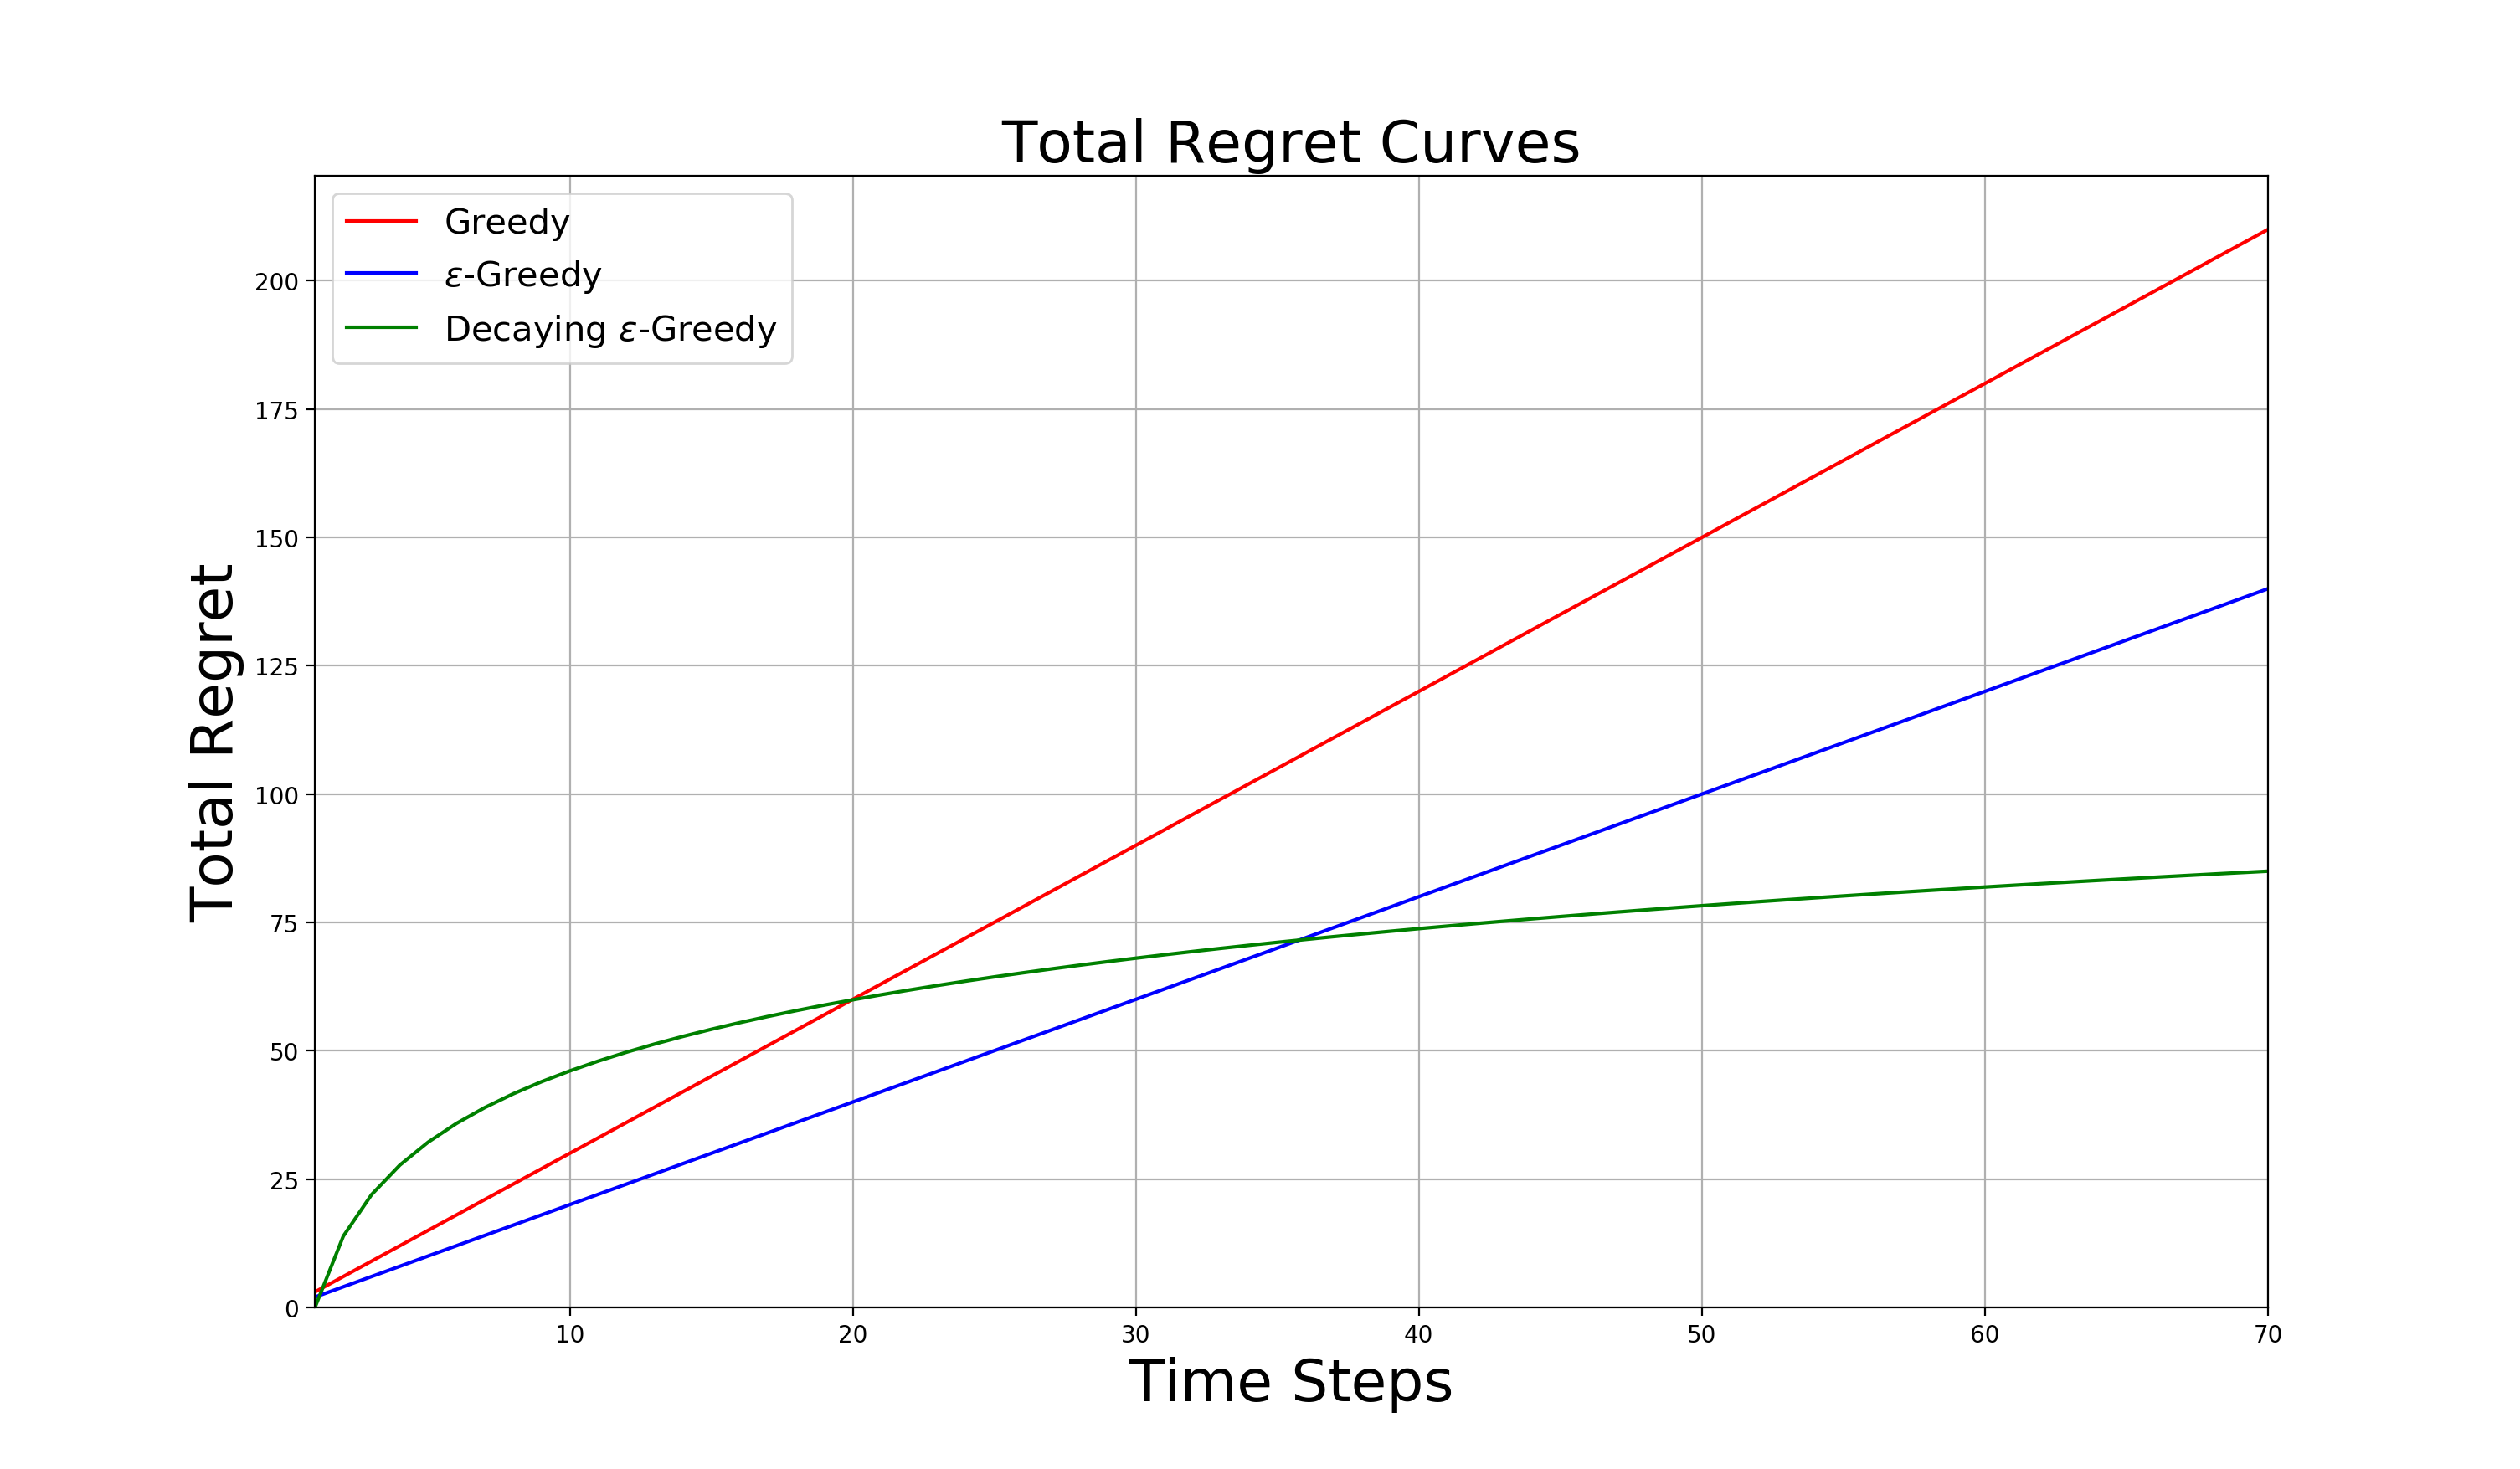
\includegraphics[width=0.62\textwidth,height=0.55\textheight,keepaspectratio]{images/bandits/figures/regret-curves.jpg}
\begin{itemize}
    \item If an algorithm never explores, it will have linear total regret
    \item If an algorithm forever explores, it will have linear total regret
    \item Is it possible to achieve sublinear total regret?
\end{itemize}
\end{frame}
